\documentclass[a4paper,titlepage,12pt]{article}
\usepackage[utf8x]{inputenc}
\usepackage[russian]{babel}
\usepackage{graphicx}
\usepackage{latexsym}
\usepackage{hyperref}
\usepackage{multirow}
\usepackage{multicol}
\usepackage{geometry}
\usepackage[version=3]{mhchem}
\usepackage{gensymb}
\usepackage[russian]{nomencl}
\usepackage{color}
\usepackage{caption2}

\graphicspath{{dot/}{gnuplot/}{gnuplot/Km/}{img/}}

\geometry{top=3cm}
\geometry{bottom=3cm}
\geometry{left=3cm}
\geometry{right=2cm}

\renewcommand{\captionfont}{\small \sffamily} % \bfseries
\renewcommand{\captionlabeldelim}{.~}

\let\originaltable\table
\let\endoriginaltable\endtable
\renewenvironment{table}[1][ht]{\originaltable[#1]\centering}
{\endoriginaltable}

\let\originalfigure\figure
\let\endoriginalfigure\endfigure
\renewenvironment{figure}[1][ht]{\originalfigure[#1]\centering}
{\endoriginalfigure}

\makenomenclature

\title{Выделение, очистка и изучение некоторых кинетических свойств альдолазы из мышц кролика.\\
    Отчет за практикум по энзимологии}
\author{Студентов четвертого курса
    Мкртчян Гарика и Нагаева Бориса}
\date{2011}

\begin{document}

\maketitle
\thispagestyle{empty}

\setcounter{page}{3}

\tableofcontents
\printnomenclature

\nomenclature{mg}{миллиграмм}
\nomenclature{ml}{миллилитр}
\nomenclature{µg}{микрограмм}
\nomenclature{µl}{микролитр}

\nomenclature{M}{моль/литр}
\nomenclature{Da}{Дальтон}
\nomenclature{альдолаза}{фруктозодифосфатальдолаза}
\nomenclature{бисфосфат}{фруктозо-1,6-дифосфат}


\newpage

\section{Введение}
Фермент фруктозодифосфатальдолаза (EC 4.1.2.13) катализирует обратимое расщепление
фруктозо-1,6-дифосфата между $C_3$ и $C_4$ с образованием диоксиацетонфосфата и глицеральдегидфосфата.
Равновесие сильно сдвинуто в направлении обратной реакции.
Данная реакция является частью гликолиза. Также фермент участвует в гликонеогенезе;
было доказано, что иногда он может функционировать как адапторный белок.

\begin{figure}[htbp]
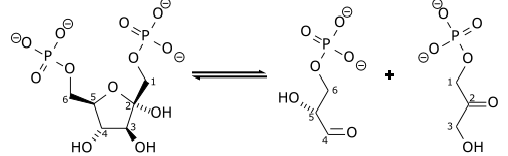
\includegraphics[width=0.8\linewidth]{intro-react}
\caption{Реакция образования глицеральдегид-3-фосфата и дигидроксиацетонфосфата}
\label{fig-intro-react}
\end{figure}

\label{lit-m}
Фермент представляет собой тетрамер, состоящий из 4 одинаковых субъединиц
($ 162 \text{kDa} = 4 \cdot 40.5 \text{kDa} $).
Животные ткани содержат по меньшей мере три различные альдолазы, характерные для
мышцы, печени и мозга (A, B, C).

\begin{figure}[htbp]
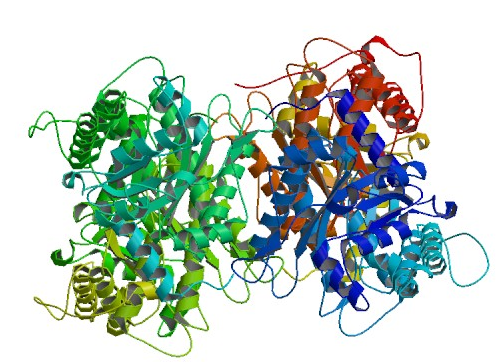
\includegraphics[width=0.8\linewidth]{intro-pdb}
\caption{Пространственная структура альдолазы А из мышц кролика,
    рисунок был взят из банка данных PDB, код - 1ZAH}
\label{fig-intro-pdb}
\end{figure}

A, B, C кодируются тремя разными генами и по-разному экспрессируются в течение развития организма
\cite{ABC} \cite{ABC-1}.
Альдолазы А и С были найдены в тканях взрослых животных.

\emph{Кинетические параментры}: для человека константа Михаэлиса Km=52 µM для фруктозо-1,6-бисфосфата
\cite{uniprot-human}.

\emph{Изоэлектрическая точка}: 6.1 \cite{pI}



\section{Приготовление веществ}

Были приготовлены и убраны в холодильник следующие вещества:
\begin{enumerate}
\item Сульфат аммония, насыщенный раствор, pH 7.5
\item ЭДТА динатриевая соль, 5 mM раствор, pH 7.5
\item 5\% раствор аммиака (готовят из концентрированного аммиака, 25\%)
\item расвор сульфата аммония со степенью насыщения 0.52,
    приготовленный на 5\%-ном растворе аммиака
\item расвор сульфата аммония со степенью насыщения 0.5,
    приготовленный на 25 mM глицил-глициновом буфере, pH 7.5
\end{enumerate}

\subsection{Доведение pH концентрированных растворов}
\label{set-pH}
В некоторые растворы нельзя погружать электрод pH-метра,
так как эти растворы настолько концентрированны, что полученное значение pH будет неточным,
а электрод может быть попорчен.
Чтобы довести pH таких растворов до требуемого значения:
\begin{enumerate}
\item отобрать небольшую пробу, например, 2 ml
\item разбавить в 20 раз
\item погрузить электрод
\item довести pH до требуемого, прикапывая кислоту или щелочь
\item чтобы довести pH исходного раствора, следует добавить
     $ \frac{2}{3} \frac{V}{2\text{ml}} V_a$ кислоты или щелочи
     ($\frac{2}{3}$ -- эмпирическая величина), где:
     $ V $ -- объем исходного раствора,
     $ V_a $ -- объем добавленной кислоты или щелочи
\end{enumerate}


\section{Выделение фермента из скелетных мышц кролика (2 сентября)}
\subsection{Экстракция}
100 g мышц кролика было разрезано ножом и ножницами на фрагменты,
длина которых не превышала 5 мм.
В гомогенизатор с металлическими ножами было добавлено 150 ml ЭДТА, 5 mM, pH 7.5.
После этого фрагменты мышцы поместили в гомогенизатор и измельчали до тех пор,
пока вещество в гомогенизаторе не стало похоже на кашу.

Смесь была перемещена в стакан, после чего добавили ещё 75 ml охлежденного 5 mM ЭДТА, pH 7.5,
и перемешали в течение 10 минут.
Гомогенат пропустили через 4 слоя марли и процентрифугировали (20 минут при 18000 g).
Супернатант собрали. Объем супернатанта составил 240 ml.
Из супернатанта отобрали 500 мкл для анализов (\emph{проба 1}).

\subsection{Фракционирование}
\label{2-frac-end}
pH раствора был доведен до 7.5.
Для этого прикапывали равный объем (240 ml) холодного 5\%-ный аммиака
с помощью делительной воронки, при интенсивном перемешивании в течении 30(FIXME) минут.
Степень насыщения стала равной 0.5.
После этого оставили на 15 минут на холоде.

Затем раствор отцентрифугировали (20 минут при 18000g).
Супернатант собрали. Объем супернатанта составил 430 ml.
Из супернатанта отобрали 500 мкл для анализов (\emph{проба 2}).

Супернатант довели до степени насыщения 0.52 добавлением
насыщенного раствора сульфата аммония, pH 7.5 (4 ml  на каждые 100 ml раствора).
pH довели до 8.0 с помощью раствора сульфата аммония со степенью насыщения 0.52,
приготовленного на 5\%-ном растворе аммиака.
Данный раствор мог повредить электрод, поэтому придерживались
техники доведения pH концентрированных растворов (см. \ref{set-pH}).

Раствор оставили на сутки в холодильнике, ожидая появления кристаллов.


Однако кристаллы альдолазы так и не выпали.
Чтобы получить кристаллы, раствор довели до комнатной температуры,
после чего поставили в холодильник. Раствор помутнел.

Затем раствор центрифугировали (20 минут при 30000g).
Объем супернатанта составил 410 ml.
Из супернатанта отобрали 500 мкл для анализов (\emph{проба 3}).
Осадок перенесли в стеклянный стаканчик путем суспендирования осадка
в растворе сульфата аммония со степенью насыщения 0.5,
приготовленного на 25 mM глицил-глициновом буфере, рН=7.5.
Затем осадок, содержащий альдолазу, поместили в холодильник (\emph{проба 4}).
Объем осадка составил примерно 8 ml.

\section{Определение концентрации белка}

\subsection{Спектрофотометрическое опредление концентраций}
$$ A_{280} = \epsilon c l $$
Проверяли, что $ 0.1 < A_{280} < 1 $.

Для всех проб действовали по следующей схеме:
\begin{enumerate}
\item набирали 2 ml бидистилированной воды в кювету
\item обнуляли прибор
\item доливали 50 µl раствора из пробы
    (данное количество было подобрано, чтобы разведение составило 41).
\item снимали значение $A_{280}$
\end{enumerate}
Таким образом, разведение равно 41.
Было допущено, что удельное поглощение $\epsilon = 1$ для белка.
Для пробы 4 было использовано литературное значение $\epsilon = 0.91$.
Толщина кюветы $l = 1 \text{cm}$.
Таким образом, концентрация белка в пробе равна [mg/ml]:
$$ c=41 \cdot A $$

\begin{table}[htbp]
\caption{Концентрация белка, определенная спектрофотометрическим способом}
\begin{tabular}{|c|c|c|}
\hline
Проба & A & C[mg/ml] \\
\hline
1 & 0.49 & 20 \\
1 & 0.54 & 22 \\
\hline
2 & 0.177 & 7.257 \\
2 & 0.2 & 8.2 \\
\hline
3 & 0.154 & 6 \\
\hline
4 & 0.148 & 32.7 \\
\hline
\end{tabular}
\end{table}

\subsection{Введение в метод Брэдфорд}
Метод Брэдфорд -- один из колориметрических методов количественного определения белков в растворе
(особенно с низкой концентрацией).
Данный метод основан на связывании белками красителя Coomassie Brilliant Blue G-250 \cite{bradford-1}.
Механизм связывания Coomassie заключается во взаимодействии анионной формы красителя с белком \cite{bradford-2}.

\begin{figure}[htbp]
\def\svgwidth{0.7\linewidth}\input{img/Coomassie_Brilliant_Blue_G-250.pdf_tex}
\caption{Краситель Coomassie Brilliant Blue G-250}
\end{figure}

Связывание с белком осуществляется за счет электростатического взаимодействия сульфонильных групп
красителя с аминокислотными остатками белка.
Связывание красителя Coomassie происходит преимущественно с аргининовым остатком и в меньшей степени с
остатками гистидина, лизина, тирозина, триптофана и фенилаланина.
Количество связей, образуемых между Coomassie и белком, зависит от количества положительно заряженных групп,
расположенных в молекуле белка.
Считается, что 1.5-3 молекулы красителя связываются одной положительно заряженной группой \cite{bradford-3}.
Исходный кислый раствор Coomassie имеет максимум поглощения при длине волны 465 нм.
После связывания с белком и изменения окраски максимум поглощения смещается к 595 нм
(рисунок~\ref{fig-shift}).

\begin{figure}[htbp]
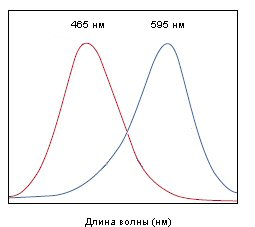
\includegraphics[width=0.4\linewidth]{bradford-shift}
\caption{Сдвиг максимума поглощения после связывания Coomasie с белком}
\label{fig-shift}
\end{figure}

\subsection{Калибровка для метода Брэдфорд}
\label{A0k}

Состав пробы: 1.9 ml Брэдфорд, буфер и БСА с концентрацией 0.4 mg/ml.

Под экспериментальные данные была подогнана линейная зависимость
(рисунок~\ref{fig-calibration}).

\begin{figure}[htbp]
\input{gnuplot/bsa}
\caption{Калибровка для метода Брэдфорд.
    На графике показана зависимость $A_{595}$ от содержания белка в кювете}
\label{fig-calibration}
\end{figure}

\subsection{Определение концентраций белка методом Брэдфорд}

Учитывая примерные концентрации, полученные спектрофотометрическим методом,
раствор из проб развели так, чтобы количество белка лежало в пределах
калибровочной кривой (0.1 -- 0.2).

Концентрация белка в пробе (mg/ml):

$$ c = \frac{m \cdot N}{V_c} $$
где $m$ -- содержание белка в кювете (µg),
$N$ -- разведение,
$V_c$ -- объем кюветы (2 ml).

\subsubsection{Проба 2}
Начали анализ с \emph{пробы 2}, в связи с чем потребовалось 4 попытки,
чтобы попасть в облась калибровочной кривой.

\def\svgwidth{\linewidth}\input{dot/br2-0.pdf_tex}

\def\svgwidth{\linewidth}\input{dot/br2-1.pdf_tex}
Содержание белка: $ m = \frac{A-A_0}{k} = 53.97 $ µg белка на кювету. \\
Разведение: $ N = 400 $ раз.
Концентарция белка в пробе: $ c = \frac{m \cdot N}{V_c} = 10.8 $ mg/ml.

\def\svgwidth{\linewidth}\input{dot/br2-2.pdf_tex}
Содержание белка: $ m = \frac{A-A_0}{k} = 35.32 $ µg белка на кювету. \\
Разведение: $ N = 1000 $ раз.
Концентарция белка в пробе: $ c = \frac{m \cdot N}{V_c} = 17.6 $ mg/ml.

\def\svgwidth{\linewidth}\input{dot/br2-3.pdf_tex}
Содержание белка: $ m = \frac{A-A_0}{k} = 25.07 $ µg белка на кювету. \\
Разведение: $ N = 2000 $ раз.
Концентарция белка в пробе: $ c = \frac{m \cdot N}{V_c} = 25.1 $ mg/ml.

Последние два опыта привели к желаемому результату
(A находится в области калибровочной прямой).

\subsubsection{Проба 1}
\def\svgwidth{\linewidth}\input{dot/br1.pdf_tex}
Содержание белка: $ m = \frac{A-A_0}{k} = 7.8 $ µg белка на кювету. \\
Разведение: $ N = 4000 $ раз.
Концентарция белка в пробе: $ c = \frac{m \cdot N}{V_c} = 15.6 $ mg/ml.

\subsubsection{Проба 3}
\def\svgwidth{\linewidth}\input{dot/br3.pdf_tex}
Содержание белка: $ m = \frac{A-A_0}{k} = 6.2 $ µg белка на кювету. \\
Разведение: $ N = 2000 $ раз.
Концентарция белка в пробе: $ c = \frac{m \cdot N}{V_c} = 6.2 $ mg/ml.



\section{Электрофорез (8 сентября)}

Электрофорез по Лэммли является одним из наиболее популярных методов по работе с белками. С
помощью электрофореза в полиакриламидном геле, белки можно фракционировать по молекулярной
массе, размерам и форме, так как данный метод имеет большую разрешающею способность. Преимущества
данного метода следующие: гель химически стабилен, нет электроосмоса, устойчивость к
растворителям, изменению рН и температуре.

Процесс полимеризации полиакриламидного геля представляет собой некую химическую реакцию,
мономером которой служит акриламид. Так как реакция у нас протекает по радикальному механизму, то
в качестве молекулы инициатора служит персульфат аммония (ПСА). Полимеризация начинается с
образования радикала из ПСА. Катализатором процесса служит тетраметилэтилендиамин (TEMED). Первая
реакция инициирует разрыв связи между двумя кислородами в молекуле персульфата аммония. В
результате этой реакции образуется свободный радикал с одним неспаренным электроном у атома
кислорода. Данный радикал влияет на разрыв двойной связи в молекуле акриламида. Такая цепная
реакция продолжается, пока два радикала не образуют между собой ковалентную связь.

\subsection{Подготовка белков}

Так как многие белки имеют вторичную, третичную и иногда четвертичную структуру, то следует их
предварительно денатурировать, чтобы избежать влияния структуры белка и заряда на его
подвижность в геле.  Для этого их кипятят в Sample Buffer (SB). Это буфер, который в себя включает краситель
бромфеноловый синий (позволяет нам следить за ходом процесса), глицерин (облегчает нанесение
образца на гель), SDS и $\beta$-меркаптоэтанол. SDS -- это ионный детергент (додецилсульфат натрия), который
за счет гидрофобных взаимодействий связывается с белками в соотношении 1,4 мг SDS на 1 мг белка. Так
как в растворе образуется избыток диссоциированных остатков сульфокислоты, собственный заряд
белка становится несущественным. $\beta$-меркаптоэтанол способствует разрыву дисульфидных связей в
молекуле белка. Кипячение способствует также денатурации белка. Из этого можно сделать вывод, что
в полиакриамидном геле разделение белков идет только по массе.

\subsection{Суть процесса}

Одной из особенностей данной системы ЭФ заключается в том, что у нас участвуют 2 геля --
(мелкопористый, нижний) и концентрирующий (крупнопористый, верхний). Кроме размеров
пор, эти гели отличаются по pH. В концентрирующем геле разделение белков не происходит. В нем белки
собираются в одну узкую полосу. Для разделяющего геля эта полоса будет стартом для начала
фракционирования. Смысл процесса заключается в следующем. Как только мы включаем электрическое
напряжение, напряженность электрического поля одинакова по всему гелю. Образцы начинают входить
в гель. Ионы глицина в концентрирующем геле имеют отрицательный заряди начинают замещать ионы
хлора. Следовательно, в концентрирующем геле  с более кислым pH, большинство молекул глицина
изменят заряд на нейтральный. Такая нейтрализация увеличивает напряженность электрического
тока в концентрирующем геле и образцы начнут двигаться. В разделяющем геле мы увидим обратный
эффект -- напряженности поля. Это приведет к тому, что белки начнут замедлять свое
движение. Отсюда начнется медленное разделение белков под воздействием низкой напряженности
электрического поля.

\subsection{Определение концентрации пробы 4}
Предполагалось, что в пробе 4 содержится суспензия альдолазы.
Чтобы исследовать пробу 4 методом электрофореза,
требуется знать примерную концентрацию белка в пробе.
Для этого провели ещё одно спектрофотометрическое определение концентрации.

Было отобрано 10 µl пробы и помещено в кювету объемом 2 ml.
Разведение составило 201 раз.

$$ A_{260} = 0.110 $$
$$ A_{280} = 0.148 $$

По формуле Калькара
$$ c = N (1.45 A_{280} - 0.74 A_{260} = 201 (1.45 \cdot 0.148 - 0.74 \cdot 0.110) = 26.8 \text{mg/ml}$$

Учитывая, что проба 4 считается очищенной от нуклеотидов и остальных белков,
можно применить следующую формулу:
$$ c = N \frac{A_{280}}{\epsilon l} = 201 \frac{0.148}{0.91 \cdot 1} = 32.7 \text{mg/ml}$$

Таким образом, концентрацию альдолазы в пробе 4 будем считать 32.7 mg/ml.

\subsection{Определение концентрации пробы 2}
Так как значения концентрации пробы 2 получились довольно разными,
было проведено повторное определение концентрации пробы 2 спектрофотометрическим методом.

Было отобрано 80 µl пробы и помещено в кювету объемом 2 ml.
Разведение составило 26 раз.

$$ A_{260} = 0.526 $$
$$ A_{280} = 0.343 $$

По формуле Калькара
$$ c = N (1.45 A_{280} - 0.74 A_{260} = 26 (1.45 \cdot 0.343 - 0.74 \cdot 0.526) = 2.8 \text{mg/ml}$$

\subsection{Исходные концентрации проб}
После рассмотрения концентраций проб, полученных спектрофотометрическим методом
и методом Брэдфорд, было обнаружено, что точность концентрации пробы 2 вызывает
сомнения.

Значения концентрации пробы 3, полученные обоими методами, почти совпали (6 mg/ml).
Концентрация пробы 1 принята за 15.6 mg/ml.
Концентрация пробы 2 должна быть меньше концентрации пробы 1
(уже потому, что объем, из которого отбиралась проба 1,
меньше объема, из которого отбиралась проба 2).
В то же время, концентрация пробы 2 должна быть больше концентрации пробы 3,
так как проба 3 отбиралась из раствора, из которого была удалена альдолаза.
Учитывая эти соображения, решили, что концентрация пробы 2 равна 10.8 mg/ml.

\subsection{Разбавление белковых проб}
Известно, что для использования пробы в электрофорезе концентрация
белка должна быть примерно 0.5 mg/ml.
Объем образца для электрофореза: 200 µl.
Было решено сначала разбавить все пробы в 5 раз, после чего
отобрать из них объем, необходимый для электрофореза.

Чтобы получить образец с концентрацией 0.5 mg/ml,
из раствора, полученного разбавлением пробы в 5 раз,
необходимо отобрать
$$ V = N \frac{C_2 V_2}{C_1} = 5 \frac{0.5 \text{mg/ml} \cdot 0.2 \text{ml}}{C_1} = \frac{0.5}{C_1} \text{[ml]} $$
где $C_1$ -- концентрация белка в пробе.

Рассчитаем объемы, которые нужно отбирать из разбавленных в 5 раз проб:

\begin{tabular}{|c|c|c|}
\hline
Проба & $C_1$ [mg/ml] & $V$ [µl] \\
1 & 15.6  & 32.05 \\
2 & 10.8  & 46.3  \\
3 & 6.2   & 80.65 \\
4 & 32.7  & 18.7  \\
\hline
\end{tabular}

\subsection{Приготовление образцов для электрофореза}
4-х кратный буфер для образцов (SB) был выдан преподавателем.
Для получения однократного буфера, 4-х кратных буфер был разбавлен в 4 раза.
В 1 мл SB было добавлено 50 µl меркаптоэтанола,
концентрация меркаптоэтанола в полученном буфере 5\%.
Для получения образцов для электрофореза сначала добавляли воду,
затем пробу белка, разведенную в 5 раз, затем 50 µl SB.

\begin{tabular}{|c|c|c|c|}
\hline
Проба & \ce{H20} & Проба/5 & SB \\
1 & 118 & 32   & 50 \\
2 & 104 & 46   & 50 \\
3 &  70 & 80   & 50 \\
4 & 131 & 18.7 & 50 \\
\hline
\end{tabular}

\subsection{Маркеры для электрофореза}
\begin{enumerate}
\item Phosphorilase B, 97 kDa
\item BSA, 66.2 kDa
\item Ovalbumin, 45 kDa
\item Carbonie anhydrase, 31 kDa
\item Trypsin inhibitor, 21.5 kDa
\item Lysozime, 14.4 kDa
\end{enumerate}
Оптимум нанесения: 3--5 µl на дорожку.
Хранение при -20\celsius.

\subsection{Проведение электрофореза}
В 10 лунок геля были нанесены образцы:
\begin{enumerate}
\item маркер
\item проба 1 (8 µl, 4 µg)
\item проба 2 (8 µl, 4 µg)
\item проба 3 (8 µl, 4 µg)
\item проба 4 (8 µl, 4 µg)
\item пустая
\item проба 1 (16 µl, 8 µg)
\item проба 2 (16 µl, 8 µg)
\item проба 3 (16 µl, 8 µg)
\item проба 4 (16 µl, 8 µg)
\end{enumerate}

Параметры электрофореза: 20 mA, 400 V.

\subsection{Результаты электрофореза}
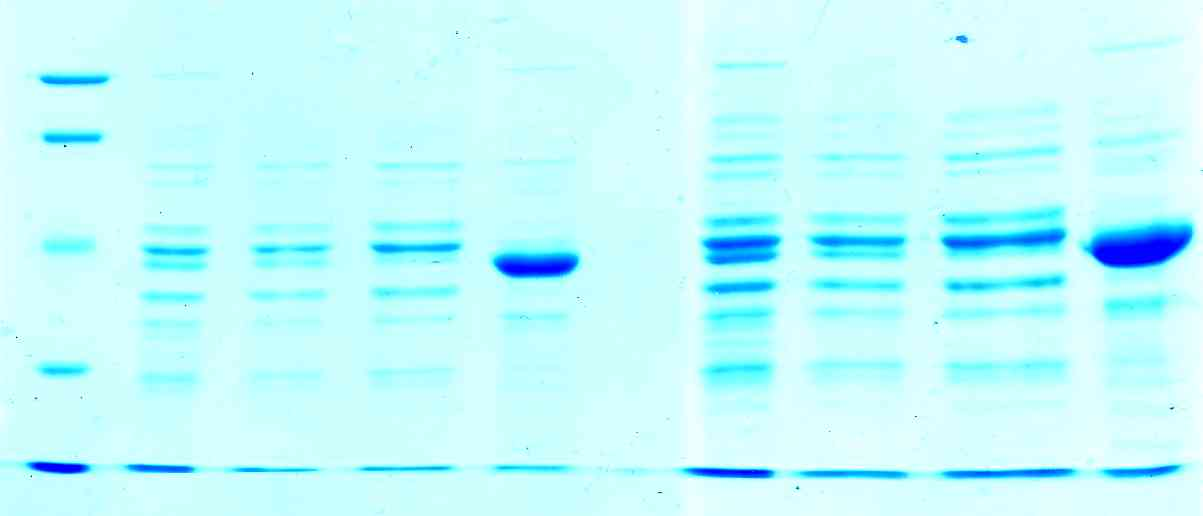
\includegraphics[width=\linewidth]{ef.jpg}

\emph{Вывод}: последняя стадия эффективно отделила альдолазу.



\subsection{Маркеры для электрофореза: SM0671}
\begin{enumerate}
\item 170 kDa
\item 130 kDa
\item 95 kDa
\item 72 kDa -- красный
\item 55 kDa
\item 43 kDa
\item 34 kDa
\item 26 kDa
\item 17 kDa
\item 10 kDa -- желтый
\end{enumerate}

\subsection{Проведение электрофореза}
В 10 лунок геля были нанесены образцы:
\begin{enumerate}
\item маркер
\item проба 1 (8 µl, 4 µg)
\item проба 2 (8 µl, 4 µg)
\item проба 3 (8 µl, 4 µg)
\item проба 4 (8 µl, 4 µg)
\item пустая
\item маркер
\end{enumerate}

Параметры электрофореза: 20 mA, 400 V.

\def\svgwidth{0.7\linewidth}\input{img/ef-2.pdf_tex}

\subsection{Вычисление массы выделенного белка}
Выделенный белок немного легче маркера 6, имеющего массу 43 kDa.
Это согласуется с литературными данными (см. \ref{lit-m}).

\input{gnuplot/ef}

M = 40.9 Da

Данное значение согласуется с литературными данными (см. \ref{lit-m}).

\emph{Вывод}: последняя стадия эффективно отделила альдолазу.



\section{Определение активности альдолазы}

Решили измерять активность по NADH.

\def\svgwidth{0.7\linewidth}\input{dot/NADH.pdf_tex}

\subsection{Приготовление растворов}

\subsubsection{Глицил-глициновый буфер}
$$ \text{m} = M \cdot c \cdot V =
    132.12 \text{Da} \cdot 0.05 \text{M} \cdot 0.1 \text{l} = 0.6606 \text {g} $$
pH раствора был доведен до 7.5.

\subsubsection{NADH}
$$ \text{m} = M \cdot c \cdot V =
    763 \text{Da} \cdot 0.02 \text{M} \cdot 0.001 \text{l} = 0.01526 \text {g} $$

\subsubsection{Соль фруктозобисфосфата}
\label{bisphosphate}
$$ \text{m} = M \cdot c \cdot V =
    378 \text{Da} \cdot 0.075 \text{M} \cdot 0.001 \text{l} = 0.02837 \text {g} $$

\subsubsection{Коммерческий препарат ферментов}
Коммерческий препарат ферментов, содержащий триозофосфатизомеразу и
глицерол-3-фосфат-дегидрогеназу.
Концентрация рабочего раствора составила 6.3 mg/ml.
Активность глицерол-3-фосфат-дегидрогеназы: 150 E/ml.
Активность триозофосфатизомеразы: 1.6 E/ml.
Раствор был приготовлен на 50 mM глицил-глициновом буфере.

\subsubsection{Фруктозобисфосфатальдолаза}
Раствор был приготовлен на 50 mM глицил-глициновом буфере.

\subsection{Измерение активности}
\label{activeness}
Для измерения активности значения $A_{340}$ снимают каждые 30 секунд
в течении как минимум 3 минут.
\begin{enumerate}
\item добавить 1.9 ml глицил-глицинового буфера
\item 25 µl вспомогательных ферментов
\item альдолаза
\item поместить кювету в прибор и обулить
\item добавить 15 µl NADH
\item добавить бисфосфат на палочке и перемешать этой же палочкой
\item запустить прибор
\end{enumerate}

При измерения активности изменяли объем вносиной альдолазы,
при измерении $K_M$ -- объем бисфосфата (субстрата альдолазы).
При измерения активности объем добавляемого
бисфосфата оставался постоянным (60 µl).

\subsection{Пробные опыты}

NADH вносят так, чтобы значение A после добавления NADH
было около 0.8

В первую попытку внесли 2 ml буфера и 30 µl NADH.
Значение A составило 1.484.
Это значение слишком велико.

В второй раз (и в последующие разы) вносили по 15 µl NADH и
30 µl альдолазы из пробы 4.
Однако такое количество альдолазы слишком быстро израсходовало
весь субстрат.

Альдолазу из пробы 4 разбавили в 100 раз (10 µl альдолазы в 1 ml воды).
В третий раз отобрали 30 µl разбавленной альдолазы.
Отсчет времени запустили после добавления NADH.
Получилась довольно странная зависимость
(D было низким до добавления субстрата, а затем выросло).
По-видимомму, это вызвано тем, что отсчет времени был включен до перемешивания.

В четвертый раз внесли 20 µl альдолазы (начиная с этого опыта, вносили разравленную альдолазу).
Получилась хорошая зависимость.
Однако решили снимать показания в течении 5 минут.

\input{gnuplot/9-1}

\subsection{Снятие активности при разных концентрациях альдолазы}
Была проведена серия экспериментов (см. \ref{activeness}).
При этом концентрация субстрата оставалась неизменной (60 µl).
Литературное значение $K_M = 52 µM$.
При добавлении бисфосфата в кювету его концентрация снижалась в $\frac{2000}{60} = 33$ раз.
Исходная концентрация бисфосфата равна 75 mM.
Значит, концентрация бисфосфата в кювете около $\frac{75}{33} = 2.3$ mM,
что намного превышает $K_M$.
Так как насыщающей концентрацией можно считать концентрацию 10--20 $K_M$,
используемая концентрация наверняка являлась насыщающей.

Используемые объемы (разбавленной) альдолазы: 20 µl, 10 µl и 5 µl.
Показания прибора снимались в течении 5 минут.
Были получены следующие зависимости:

\input{gnuplot/9-2}

Зависимости пересчитали на $\Delta D$, которое пропорционально количеству израсходованного субстрата.
$\Delta D$ рассчитывали, как разность исходного и текущего значений D.
Кроме того, рассматривали зависимость, спустя 2 минуты от начала отсчета,
так как до 2 минут реакция, кажется, находится в лаг-фазе.

\input{gnuplot/9-2-d}

Зависимости спрямили. Значения $\frac{\Delta D}{\text{min}}$:

\begin{tabular}{|c|c|}
\hline
$ V_{\text{альдолазы}} $ & $ \Delta D / \text{min} $ \\
\hline
20 & 0.172 \\
10 & 0.087 \\
05 & 0.045 \\
\hline
\end{tabular}

По данным точкам построили график:

\input{gnuplot/9-2-D}

Содержание (в mg) альдолазы в кювете можно получить по следующей формуле:
$$ m = \frac{1}{100} V_\text{альдолазы} \cdot 32.7 \text{mg/ml} $$
По оси абсцисс отложено содержание (в mg) альдолазы в кювете.
Объемы добавляемой альдолазы (20, 10 и 5 µl) отмечены внутри графика.

После спрямления зависимости выяснилось, что
$\frac{\Delta D}{\text{min} \cdot {mg альдолазы}} = 25.9$.

Вычислим активность альдолазы:
$$ E = \frac{1}{2} \frac{\Delta D_{340} \cdot V_{кюветы}}{\text{мин} \cdot 6.22 \cdot \text{mg альдолазы}} =
    \frac{1}{2} 25.9 \cdot \frac{2 ml}{6.22} = 4.2 \frac{µmol}{\text{mg} \cdot \text{мин}} $$
$\frac{1}{2}$ в формуле, так как на одну израсходованную молекулу субстрата
расходуется две молекулы NADH.

Активность альдолазы довольно высока, что подтверждает высокое качество
проведенного выделения.



\section{Вычисление чистоты субстрата}
Чтобы вычисление константы Михаэлиса было более точным, провели
эксперимент для вычисления чистоты субстрата.
Для этого измерили A сразу после добавления NADH, до добавления субстрата.
Значение A составило 0.805.

Количество добавленного субстрата: 10 µl, разбавление в 10 раз.

Значение A стало снижаться, после чего вышло на плато на уровне 0.5.

$$ \Delta D = 0.305 $$
$$ \Delta \nu\text{NADH} = \frac{\Delta D \cdot V_\text{кюветы}}{6.22} = 0.098 \text{µmol} $$
$$ \nu S = \frac{1}{2} \Delta \nu\text{NADH} = 0.049 \text{µmol} $$

$\frac{1}{2}$ в формуле, так как на одну израсходованную молекулу субстрата
расходуется две молекулы NADH.

$$ C_\text{S в кювете} = \frac{\nu S}{V_\text{кюветы}} = \frac{0.049}{2} = 0.0245 mM $$
$$ C_S = C_\text{S в кювете} \cdot N = 0.0245 M \cdot 200 \cdot 10 = 49 mM $$
$$ \text{чистота} = \frac{49 mM}{75 mM} = 0.65 (65 \%) $$


\section{Измерение Км}

Была проведена серия экспериментов, описанных в \ref{activeness}.
При этом количество альдолазы оставалось постоянным (10 µl, разбавленная в 100 раз),
а количество бисфосфата изменялось.

Схема разбавления бисфосфата представлена на рисунке~\ref{km-dilution}

\begin{figure}[htbp]
\def\svgwidth{\linewidth}\section{Измерение Км (10 сентября)}

Была проведена серия экспериментов, описанных в \ref{activeness}.
При этом количество альдолазы оставалось постоянным (10 µl, разбавленная в 100 раз),
а количество бисфосфата изменялось.

\def\svgwidth{\linewidth}\section{Измерение Км (10 сентября)}

Была проведена серия экспериментов, описанных в \ref{activeness}.
При этом количество альдолазы оставалось постоянным (10 µl, разбавленная в 100 раз),
а количество бисфосфата изменялось.

\def\svgwidth{\linewidth}\input{dot/10.pdf_tex}

\begin{tabular}{|c|c|c|c|c|}
\hline
Время &  80  & 40    &  20   &  10   \\
\hline
0:00 & 1.201 & 0.853 & 0.876 & 0.864 \\
0:30 & 1.176 & 0.824 & 0.847 & 0.840 \\
1:00 & 1.146 & 0.784 & 0.807 & 0.806 \\
1:30 & 1.105 & 0.742 & 0.764 & 0.767 \\
2:00 & 1.064 & 0.698 & 0.719 & 0.724 \\
2:30 & 1.022 & 0.653 & 0.673 & 0.679 \\
3:00 & 0.980 & 0.608 & 0.627 & 0.635 \\
3:30 & 0.937 & 0.564 & 0.580 & 0.591 \\
\hline
\end{tabular}

\begin{tabular}{|c|c|c|c|c|c|c|}
\hline
Время &  100   &  80   &  60   &  40   &  20   &  10   \\
\hline
0:00  &  0.847 & 0.887 & 0.852 & 0.858 & 0.859 & 0.863 \\
0:30  &  0.823 & 0.816 & 0.828 & 0.838 & 0.835 & 0.838 \\
1:00  &  0.791 & 0.784 & 0.799 & 0.808 & 0.804 & 0.804 \\
1:30  &  0.753 & 0.745 & 0.766 & 0.773 & 0.766 & 0.765 \\
2:00  &  0.714 & 0.704 & 0.730 & 0.737 & 0.723 & 0.726 \\
2:30  &  0.674 & 0.661 & 0.692 & 0.698 & 0.681 & 0.684 \\
3:00  &  0.632 & 0.619 & 0.652 & 0.657 & 0.638 & 0.644 \\
3:30  &  0.590 & 0.576 & 0.610 & 0.617 & 0.596 & 0.606 \\
\hline
\end{tabular}

\begin{tabular}{|c|c|c|c|c|c|c|}
\hline
Время & 100   &  80   &   60  & 40   & 20   &  10  \\
\hline
0:00  & 0.796 & 0.837 & 0.865 &0.849 &0.858 &0.882 \\
0:30  & 0.773 & 0.814 & 0.847 &0.829 &0.837 &0.868 \\
1:00  & 0.741 & 0.783 & 0.822 &0.799 &0.817 &0.860 \\
1:30  & 0.704 & 0.748 & 0.792 &0.770 &0.806 &0.856 \\
2:00  & 0.665 & 0.713 & 0.761 &0.747 &0.805 &0.855 \\
2:30  & 0.626 & 0.676 & 0.732 &0.735 &0.799 &0.855 \\
3:00  & 0.587 & 0.645 & 0.706 &0.728 &0.798 &0.856 \\
3:30  & 0.550 & 0.625 & 0.687 &0.726 &0.799 &0.857 \\
\hline
\end{tabular}

\begin{tabular}{|c|c|c|}
\hline
Координаты & Km, µM & Vm, $\frac{\Delta D}{\text{min}}$ \\
\hline
Прямые, $V(S)$ & 1.91 & 0.094 \\
Обратные, $\frac{1}{V}(\frac{1}{S})$ & 0.23 & 1607 \\
Hanes, $\frac{S}{V}(S)$ & 3.64 & 0.093 \\
Eadie-Hofstee, $V(\frac{V}{S})$ & 0.49 & 0.074 \\
\hline
\end{tabular}

\input{gnuplot/10-Km-direct}

\input{gnuplot/10-Km-reverse}

\input{gnuplot/10-Km-hanes}

\input{gnuplot/10-Km-eh}



\begin{tabular}{|c|c|c|c|c|}
\hline
Время &  80  & 40    &  20   &  10   \\
\hline
0:00 & 1.201 & 0.853 & 0.876 & 0.864 \\
0:30 & 1.176 & 0.824 & 0.847 & 0.840 \\
1:00 & 1.146 & 0.784 & 0.807 & 0.806 \\
1:30 & 1.105 & 0.742 & 0.764 & 0.767 \\
2:00 & 1.064 & 0.698 & 0.719 & 0.724 \\
2:30 & 1.022 & 0.653 & 0.673 & 0.679 \\
3:00 & 0.980 & 0.608 & 0.627 & 0.635 \\
3:30 & 0.937 & 0.564 & 0.580 & 0.591 \\
\hline
\end{tabular}

\begin{tabular}{|c|c|c|c|c|c|c|}
\hline
Время &  100   &  80   &  60   &  40   &  20   &  10   \\
\hline
0:00  &  0.847 & 0.887 & 0.852 & 0.858 & 0.859 & 0.863 \\
0:30  &  0.823 & 0.816 & 0.828 & 0.838 & 0.835 & 0.838 \\
1:00  &  0.791 & 0.784 & 0.799 & 0.808 & 0.804 & 0.804 \\
1:30  &  0.753 & 0.745 & 0.766 & 0.773 & 0.766 & 0.765 \\
2:00  &  0.714 & 0.704 & 0.730 & 0.737 & 0.723 & 0.726 \\
2:30  &  0.674 & 0.661 & 0.692 & 0.698 & 0.681 & 0.684 \\
3:00  &  0.632 & 0.619 & 0.652 & 0.657 & 0.638 & 0.644 \\
3:30  &  0.590 & 0.576 & 0.610 & 0.617 & 0.596 & 0.606 \\
\hline
\end{tabular}

\begin{tabular}{|c|c|c|c|c|c|c|}
\hline
Время & 100   &  80   &   60  & 40   & 20   &  10  \\
\hline
0:00  & 0.796 & 0.837 & 0.865 &0.849 &0.858 &0.882 \\
0:30  & 0.773 & 0.814 & 0.847 &0.829 &0.837 &0.868 \\
1:00  & 0.741 & 0.783 & 0.822 &0.799 &0.817 &0.860 \\
1:30  & 0.704 & 0.748 & 0.792 &0.770 &0.806 &0.856 \\
2:00  & 0.665 & 0.713 & 0.761 &0.747 &0.805 &0.855 \\
2:30  & 0.626 & 0.676 & 0.732 &0.735 &0.799 &0.855 \\
3:00  & 0.587 & 0.645 & 0.706 &0.728 &0.798 &0.856 \\
3:30  & 0.550 & 0.625 & 0.687 &0.726 &0.799 &0.857 \\
\hline
\end{tabular}

\begin{tabular}{|c|c|c|}
\hline
Координаты & Km, µM & Vm, $\frac{\Delta D}{\text{min}}$ \\
\hline
Прямые, $V(S)$ & 1.91 & 0.094 \\
Обратные, $\frac{1}{V}(\frac{1}{S})$ & 0.23 & 1607 \\
Hanes, $\frac{S}{V}(S)$ & 3.64 & 0.093 \\
Eadie-Hofstee, $V(\frac{V}{S})$ & 0.49 & 0.074 \\
\hline
\end{tabular}

\input{gnuplot/10-Km-direct}

\input{gnuplot/10-Km-reverse}

\input{gnuplot/10-Km-hanes}

\input{gnuplot/10-Km-eh}


\caption{Схема разбавления бисфосфата для измерения $K_M$.
    На схеме отмечены отбираемые объемы (в µl) и
    концентрации полученных растворов (в mM).}
\label{km-dilution}
\end{figure}

Когда $K_M$ измеряли в первый раз, оказалось,
что полученные данные слишком шумные,
только 3 точки пришлось на <<спуск>> графика Михаэлиса-Ментен.
Поэтому измерение Km было переделано.

Действовали по прежней схеме, но:
\begin{enumerate}
\item сначала провели измерения при самых больших и самых низких концентрациях субстрата,
    после чего придерживались бинарного поиска.
    По-видимому, благодаря этому удалось избежать длительного изучения точек на плато;
\item подогрели буфер;
\item использовали натриевую соль фруктозобисфосфата (M = 340 Da) (см \ref{bisphosphate}).
\end{enumerate}

В таблице~\ref{table-s-to-v} представлена зависимость скорости реакции
от концентрации субстрата (бисфосфата).

\begin{table}[htbp]
\caption{Зависимость скорости реакции от концентрации субстрата}
\begin{tabular}{|c|c|c|c|}
\hline
S [µM] &
V [delta D/min] &
V [µmol S/min] &
V [µmol NADH/min] \\
\hline
2437  & 0.062 &  0.00997 & 0.01994 \\
1462  & 0.061 &  0.00980 & 0.01961 \\
243.7 & 0.060 &  0.00964 & 0.01929 \\
121.8 & 0.059 &  0.00948 & 0.01897 \\
60.93 & 0.052 &  0.00836 & 0.01672 \\
24.37 & 0.045 &  0.00723 & 0.01447 \\
18.2  & 0.041 &  0.00659 & 0.01318 \\
12.18 & 0.035 &  0.00562 & 0.01125 \\
8.531 & 0.021 &  0.00337 & 0.00675 \\
6.097 & 0.011 &  0.00177 & 0.00354 \\
2.437 & 0.004 &  0.00064 & 0.00129 \\
\hline
\end{tabular}
\label{table-s-to-v}
\end{table}

Значение A трех последних точек слишком низкое.
Эти точки были исключены из дальнейшего рассмотрения.
На рисунках~\ref{km-direct}, \ref{km-reverse}, \ref{km-hanes} и \ref{km-eh}
представлена зависимость скорости от концентрации субстрата (бисфосфата)
в различных координатах, а также линия аппроксимации и значения $K_M$ и $V_M$.
В таблице~\ref{table-km-and-vm} информация $K_M$ и $V_M$ собрана воедино.

\begin{figure}[htbp]
\input{gnuplot/Km/direct-17-1}
\caption{Кинетический график.
    Прямые координаты.}
\label{km-direct}
\end{figure}

\begin{figure}[htbp]
\input{gnuplot/Km/reverse-17-1}
\caption{Кинетический график.
    Координаты Лайнуивера-Берка.}
\label{km-reverse}
\end{figure}

\begin{figure}[htbp]
\input{gnuplot/Km/hanes-17-1}
\caption{Кинетический график.
    Координаты Хэйнса.}
\label{km-hanes}
\end{figure}

\begin{figure}[htbp]
\input{gnuplot/Km/eh-17-1}
\caption{Кинетический график.
    Координаты Еди-Хофсти.}
\label{km-eh}
\end{figure}

\begin{table}[htbp]
\caption{Значения $K_M$ и $V_M$}
\begin{tabular}{|c|c|c|}
\hline
Координаты & Km, µM & Vm, $\frac{\text{µmol} S}{\text{min}}$ \\
\hline
Прямые,           $V(S)$                       & 9.44 & 0.00997 \\
Лайнуивера-Берка, $\frac{1}{V}(\frac{1}{S})$   & 9.38 & 0.00996 \\
Хэйнса,           $\frac{S}{V}(S)$             & 10.2 & 0.00997 \\
Еди-Хофсти,       $V(\frac{V}{S})$             & 9.4  & 0.00996 \\
\hline
По литературным данным, для человека \cite{uniprot-human}
                                               & 52 & \\
\hline
\end{tabular}
\label{table-km-and-vm}
\end{table}

Значения Km, полученные в разных координатах, хорошо согласуются между собой
и несильно отличаются от литературных значений (отличие меньше, чем на порядок).



\newpage
\section{Выводы}
В данной работе была проведена очистка и частичная характеристика фермента
фруктозо-1,6-бисфосфатальдолазы из мышц кролика (8 ml, 32.7 mg/ml).
Студенты ознакомились с методом экстракции,
фракционирования, электрофореза и
определения кинетических параметров фермента.
Для фермента определили
молекулярную массу (40.9~kDa),
чистоту (65\%),
активность $4.2 \frac{µmol}{\text{mg} \cdot \text{min}}$ и
константу Михаэлиса (около 9.5~µM).


\begin{thebibliography}{WW}
\bibitem{pI} \url{http://www.worthington-biochem.com/ald/default.html}
\bibitem{ABC} Anderson, P., Gibbons, I., and Perham, R.:
    A Comparative Study of the Structure of Muscle Fructose 1,6-Diphosphate Aldolases,
    Eur J Biochem 11, 503, 1969
\bibitem{ABC-1}  Lai, C.Y., Nakai, N. and Chang, D. (1974)
    Amino acid sequence of rabbit muscle aldolase and the structure of the active center.
    Science 183: 1204-1206.
\bibitem{bradford-1} Bradford, M.M. (1976).
    A rapid and sensitive method for the quantitation of microgram quantities of
    protein utilizing the principle of protein-dye binding. Anal. Biochem. 72, 248-254.
\bibitem{bradford-2} Compton, S.J. and Jones, C.G. (1985).
    Mechanism of dye response and interference in the Bradford protein assay.
    Anal. Biochem. 151(2), 369-374
\bibitem{bradford-3} Tal, M., Silberstein, A. and Nusser, E. (1980).
    Why does Coomassie Brilliant Blue\textregistered interact differently with different proteins?
    J. Biol. Chem. 260, 9976-9980
\end{thebibliography}



\end{document}

